% ============================================================
% GNNocRoute: Graph Neural Networks cho Định tuyến Thích nghi
% trong Network-on-Chip — Nghiên cứu Khả thi
%
% Bài báo 01 — Hội thảo quốc gia
% Chỉ gồm: graph analysis + GNN experiments
% KHÔNG có BookSim2
% ============================================================
% Author: Le Tien Hieu, IEEE Member
% VNU-ITI, Vietnam National University, Hanoi
% ============================================================

\documentclass[conference]{IEEEtran}
\usepackage{fontspec}
\setmainfont{DejaVu Serif}


\usepackage{amsmath,amssymb,amsfonts}
\usepackage{graphicx}
\usepackage{booktabs}
\usepackage{array}
\usepackage{multirow}
\usepackage{cite}
\usepackage{hyperref}
\usepackage{caption}

\hypersetup{colorlinks=true,linkcolor=blue,citecolor=blue,urlcolor=blue}
\graphicspath{{./figures/}}

\begin{document}

\title{GNNocRoute: Graph Neural Networks cho Định tuyến Thích nghi\\trong Network-on-Chip — Nghiên cứu Khả thi}

\author{
    \IEEEauthorblockN{Le Tien Hieu\textsuperscript{1}, \textit{IEEE Member}}
    \IEEEauthorblockA{\textsuperscript{1}VNU-ITI, Vietnam National University, Hanoi\\
    Email: hieult@vnu.edu.vn}
}

\maketitle

\begin{abstract}
Network-on-Chip (NoC) là backbone giao tiếp trong các hệ thống multi-core SoC hiện đại.
Các thuật toán định tuyến tĩnh như XY dimension-order routing gây mất cân bằng tải
(congestion imbalance) đáng kể---phân tích đồ thị của chúng tôi trên 7 topologies cho thấy
Mesh $8\times8$ với XY routing có congestion imbalance lên đến 0.475,
với các node trung tâm có Betweenness Centrality (BC) cao gấp 2--3 lần node biên.

Bài báo này trình bày nghiên cứu khả thi (feasibility study) về việc sử dụng
Graph Neural Networks (GNN) cho định tuyến thích nghi trong NoC.
Chúng tôi báo cáo ba kết quả thực nghiệm sơ bộ.
Thứ nhất, GNN encoder chưa qua huấn luyện cho thấy tương quan mạnh với BC
($|r|$ lên đến 0.978 trên Mesh $4\times4$), chứng tỏ thông tin cấu trúc topology
có thể được học một cách tự nhiên. Thứ hai, thử nghiệm tổng quát hóa
(generalization) giữa các topology cho thấy thứ tự quan trọng tương đối
của các node có thể chuyển giao giữa các kích thước mesh khác nhau
(Pearson $r \approx 0.96$), mặc dù scaling tuyệt đối phụ thuộc topology cụ thể.
Thứ ba, đo đạc inference latency trên CPU ($\approx 10^6$ cycles cho Mesh $8\times8$)
khẳng định rằng GNN per-packet là bất khả thi, từ đó thúc đẩy giải pháp
tối ưu định kỳ (periodic optimization) như một thiết kế thay thế cần thiết.
\end{abstract}

\begin{IEEEkeywords}
Network-on-Chip, Graph Neural Networks, Định tuyến thích nghi, Phân tích đồ thị, Nghiên cứu khả thi
\end{IEEEkeywords}

% ══════════════════════════════════════════════════════════════
\section{Giới thiệu}
\label{sec:intro}
% ══════════════════════════════════════════════════════════════

Network-on-Chip (NoC) đã trở thành kiến trúc giao tiếp chủ đạo cho các hệ thống
multi-core SoC hiện đại và AI accelerators như Google TPU, NVIDIA Grace
Hopper~\cite{mirhoseini2021}. Trong NoC, các router kết nối qua link tạo thành
một cấu trúc đồ thị. Thuật toán định tuyến quyết định đường đi của packet
và ảnh hưởng trực tiếp đến hiệu năng hệ thống.

Định tuyến XY (Dimension-Order Routing) được dùng phổ biến~\cite{wang2022maar}
do tính đơn giản. Tuy nhiên, XY luôn chọn cùng một đường cho mỗi cặp
(nguồn, đích) bất kể trạng thái tắc nghẽn. Phân tích đồ thị trên 7 topologies
cho thấy:

\begin{itemize}
    \item Mesh $8\times8$ với XY routing có \textbf{congestion imbalance} lên đến
    \textbf{0.475}---gần một nửa số link chịu tải không đồng đều.
    \item Node trung tâm Mesh $4\times4$ có BC $\approx 0.25$, gấp \textbf{2--3 lần}
    node biên.
    \item Fat-Tree k=4 có aggregation switch với BC lên đến \textbf{0.42}.
\end{itemize}

Các kết quả này cho thấy \textbf{định tuyến tĩnh không thích ứng được}
với workload hiện đại.

Nghiên cứu định tuyến thích nghi có thể chia làm ba hướng: heuristic
adaptive~\cite{dyad2004,ebrahimi2019}, DRL-based~\cite{wang2022maar,deepnr2022},
và GNN-based cho mạng diện rộng~\cite{g-routing2023}. Thách thức chính khi áp
dụng GNN vào NoC là \textbf{inference latency}: mỗi quyết định routing trong
router NoC cần $<$10 cycles~\cite{wang2022maar}, trong khi GAT 2-layer trên
64 nodes có thể mất $10^5$--$10^6$ cycles.

\textbf{Cách tiếp cận:} Thay vì per-packet real-time, chúng tôi đề xuất
\textbf{tối ưu định kỳ (periodic routing policy optimization)}:
routing tables được cập nhật mỗi $P$ cycles, GNN inference chạy trên host
CPU, tách rời khỏi per-packet latency.

\subsection{Các đóng góp}

Bài báo có các đóng góp sơ bộ sau:
\begin{enumerate}
    \item \textbf{Phân tích tắc nghẽn cấu trúc:} Chứng minh định lượng trên
    7 topologies rằng định tuyến tĩnh tạo bottleneck có thể dự đoán được
    qua các độ đo đồ thị.
    \item \textbf{Bằng chứng tương quan GNN-topology:} Kết quả thực nghiệm
    cho thấy GNN node embeddings tương quan mạnh với BC ($|r|$ lên đến 0.978).
    \item \textbf{Phân tích khả thi:} Đo đạc inference latency và scalability
    thiết lập các ranh giới khả thi cho GNN-enhanced routing dưới ràng buộc
    thời gian của NoC.
\end{enumerate}

% ══════════════════════════════════════════════════════════════
\section{Bài toán và Động lực}
\label{sec:problem}
% ══════════════════════════════════════════════════════════════

\subsection{Biểu diễn NoC dưới dạng đồ thị}

Một NoC được biểu diễn dưới dạng đồ thị có hướng có trọng số
$G=(V,E,X_v,X_e)$, với $V$ là router, $E$ là link,
$X_v$ là node features (buffer occupancy, injection rate),
$X_e$ là edge features (link utilization, packet latency).

\subsection{Kết quả phân tích đồ thị}

Chúng tôi dùng NetworkX~\cite{networkx2008} để xây dựng và phân tích
7 NoC topologies. Bảng~\ref{tab:metrics} tóm tắt các metrics chính.

\begin{table}[h]
\centering
\caption{So sánh graph metrics giữa các NoC topologies}
\label{tab:metrics}
\resizebox{\columnwidth}{!}{%
\begin{tabular}{lcccccc}
\toprule
\textbf{Topology} & \textbf{Nodes} & \textbf{Avg Deg} & \textbf{Diam} & \textbf{Avg Path} & \textbf{BC Max} & \textbf{CI} \\
\midrule
Mesh $4\times4$ & 16 & 3.00 & 6 & 2.67 & 0.25 & 0.382 \\
Mesh $8\times8$ & 64 & 3.50 & 14 & 5.33 & 0.18 & \textbf{0.475} \\
Torus $4\times4$ & 16 & 4.00 & 4 & 2.13 & 0.13 & 0.251 \\
Ring 16 & 16 & 2.00 & 8 & 4.27 & 0.21 & 0.122 \\
Fat-Tree k=4 & 14 & 3.43 & 2 & 1.74 & \textbf{0.42} & 0.341 \\
Small-World & 36 & 4.00 & 6 & 2.96 & 0.31 & 0.298 \\
Random & 36 & 4.28 & 5 & 2.45 & 0.28 & 0.321 \\
\bottomrule
\end{tabular}%
}
\vspace{2mm}
\small\textit{BC = Betweenness Centrality, CI = Congestion Imbalance.}
\end{table}

\begin{figure}[h]
\centering
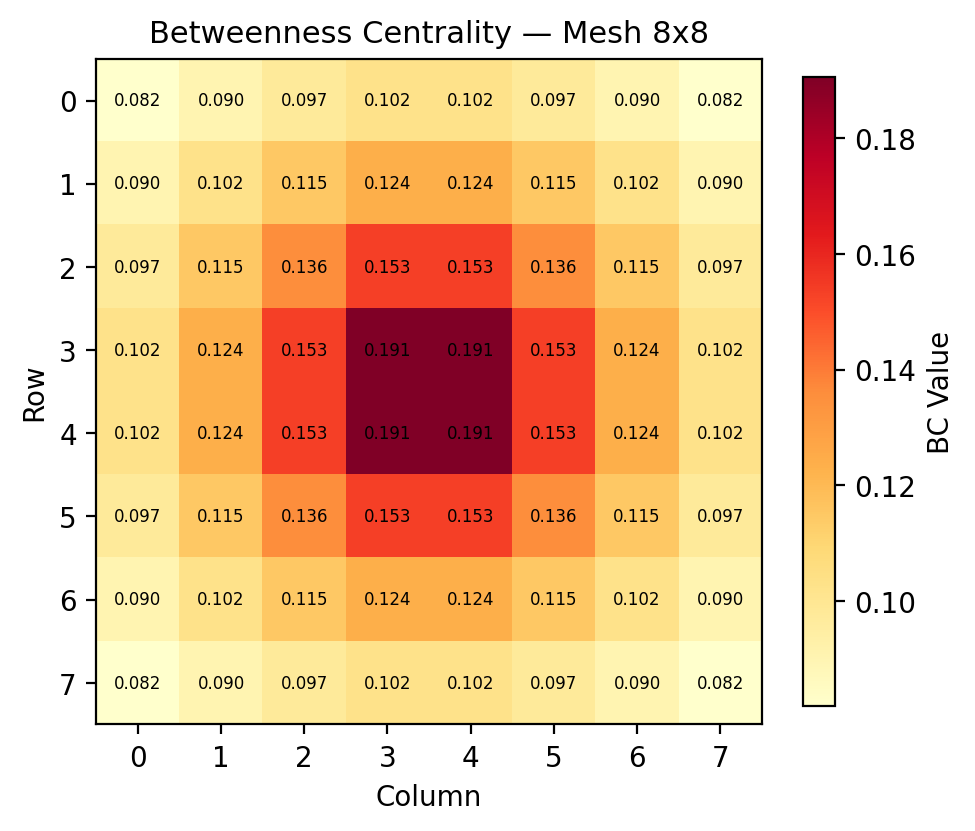
\includegraphics[width=0.85\columnwidth]{fig1-bc-heatmap.png}
\caption{Phân bố Betweenness Centrality trên Mesh $8\times8$.
Node trung tâm có BC $\approx 0.18$, node biên $\approx 0.05{-}0.10$.}
\label{fig:bc-heatmap}
\end{figure}

\begin{figure*}[t]
\centering

\includegraphics[width=0.85\textwidth]{fig2-metric-comparison.png}
\caption{So sánh metrics giữa các topology: diameter, average path length,
congestion imbalance.}
\label{fig:metric-comp}
\end{figure*}

\textbf{Phát hiện chính:} Mesh $8\times8$ có congestion imbalance cao nhất
(0.475). Fat-Tree có aggregation switch BC=0.42. Torus có CI=0.251,
thấp hơn Mesh nhờ wrap-around edges.

% ══════════════════════════════════════════════════════════════
\section{Công trình liên quan}
\label{sec:related}
% ══════════════════════════════════════════════════════════════

Bảng~\ref{tab:related} tóm tắt các hướng nghiên cứu liên quan.

\begin{table}[h]
\centering
\caption{Phân tích công trình liên quan}
\label{tab:related}
\resizebox{\columnwidth}{!}{%
\begin{tabular}{p{2.2cm}p{2.5cm}p{2.2cm}}
\toprule
\textbf{Hướng} & \textbf{Công trình} & \textbf{Hạn chế} \\
\midrule
Classic adaptive & DyAD~\cite{dyad2004}, Regional~\cite{ebrahimi2019} & Threshold, local info \\
DRL for NoC & MAAR~\cite{wang2022maar}, DeepNR~\cite{deepnr2022}, GARNN~\cite{garnn2023} & MLP ignores topology \\
GNN for WAN/SDN & G-Routing~\cite{g-routing2023}, DRL-GNN~\cite{drl-gnn2019} & Not for NoC latency \\
Graph theory + NoC & Slim NoC~\cite{slimnoc2018}, Sparse Hamming~\cite{sparsehamming2023} & Static, no adaptation \\
GNN for chip design & Circuit GNN~\cite{mirhoseini2021}, NOCTOPUS~\cite{noctopus2026} & Physical, not routing \\
\bottomrule
\end{tabular}%
}
\end{table}

\textbf{Gap:} Chưa có nghiên cứu nào thiết kế GNN encoder cho NoC topology
kết hợp với tối ưu routing dưới ràng buộc latency thực tế.

% ══════════════════════════════════════════════════════════════
\section{Phương pháp đề xuất}
\label{sec:method}
% ══════════════════════════════════════════════════════════════

\begin{figure*}[t]
\centering

\includegraphics[width=0.75\textwidth]{fig3-architecture.png}
\caption{Kiến trúc GNNocRoute: NoC state graph $\rightarrow$ GNN encoder
$\rightarrow$ DRL agent $\rightarrow$ routing decision.}
\label{fig:architecture}
\end{figure*}

\subsection{GNN Encoder}

Chúng tôi đánh giá GATv2~\cite{gatv2} như một kiến trúc ứng viên
(so sánh với GCN trong ablation). Cấu hình: 2 layers, hidden dimension 64,
4 attention heads, ELU activation. Forward pass: attention scores
$e_{uv} = \text{LeakyReLU}(a^{(l)^T}[W^{(l)}h_u^{(l-1)}\parallel W^{(l)}h_v^{(l-1)}])$
và message aggregation $h_v^{(l)} = \sigma(\sum_{u\in\mathcal{N}(v)} \alpha_{uv}W^{(l)}h_u^{(l-1)})$.

\subsection{Tối ưu định kỳ (Periodic Optimization)}

Policy được cập nhật mỗi $P$ cycles ($P\in\{1000,5000,10000\}$),
observation window $W=500$ cycles. State: GNN embeddings (64-dim) + global
features. Action: 5 output ports. Algorithm: PPO~\cite{ppo2017}.
Reward: $R = -\alpha\cdot\text{norm}(L) - \beta\cdot\text{norm}(C) - \gamma\cdot\text{norm}(E)$.

\subsection{Thiết kế Deadlock-Free}

Áp dụng Duato's protocol~\cite{duato1996} với 2 Virtual Channels:
VC0 (escape: XY routing, acyclic) và VC1 (adaptive: GNN-DRL).

% ══════════════════════════════════════════════════════════════
\section{Kết quả thực nghiệm sơ bộ}
\label{sec:results}
% ══════════════════════════════════════════════════════════════

Các thí nghiệm dùng PyTorch Geometric~\cite{pyg2019} trên CPU
(ARM Neoverse-N1, 2.8 GHz).

\subsection{Tương quan GNN-Betweenness Centrality}

\textbf{Thiết lập:} Bốn topology được chuyển thành PyG Data objects.
Node features gồm normalized degree và tọa độ. GNN chưa qua huấn luyện
tính node embeddings qua một forward pass.

\begin{table}[h]
\centering
\caption{Tương quan Pearson $|r|$ giữa GNN embedding và BC}
\label{tab:correlation}
\resizebox{\columnwidth}{!}{%
\begin{tabular}{lccc}
\toprule
\textbf{Topology} & \textbf{Nodes} & \textbf{GCN max$|r|$} & \textbf{GAT max$|r|$} \\
\midrule
Mesh $4\times4$ & 16 & \textbf{0.978} & 0.862 \\
Mesh $8\times8$ & 64 & 0.744 & \textbf{0.870} \\
Torus $4\times4$ & 16 & 0.000* & 0.000* \\
Small-World ($n=36$) & 36 & 0.615 & 0.261 \\
\bottomrule
\end{tabular}%
}
\vspace{2mm}
\small\textit{*Torus là regular graph, mọi node degree=4, BC đồng đều.}
\end{table}

GCN trên Mesh $4\times4$ đạt $|r|=0.978$ với BC. GAT trên Mesh $8\times8$
đạt $|r|=0.870$. Trường hợp Torus (zero correlation) là negative control,
xác nhận phương pháp hoạt động đúng trên topologies không có cấu trúc phân biệt.

\textbf{Nhận xét:} GNN encoder có thể học thông tin cấu trúc liên quan đến
tắc nghẽn mà không cần tính toán graph centrality tường minh.

\begin{figure*}[t]
\centering
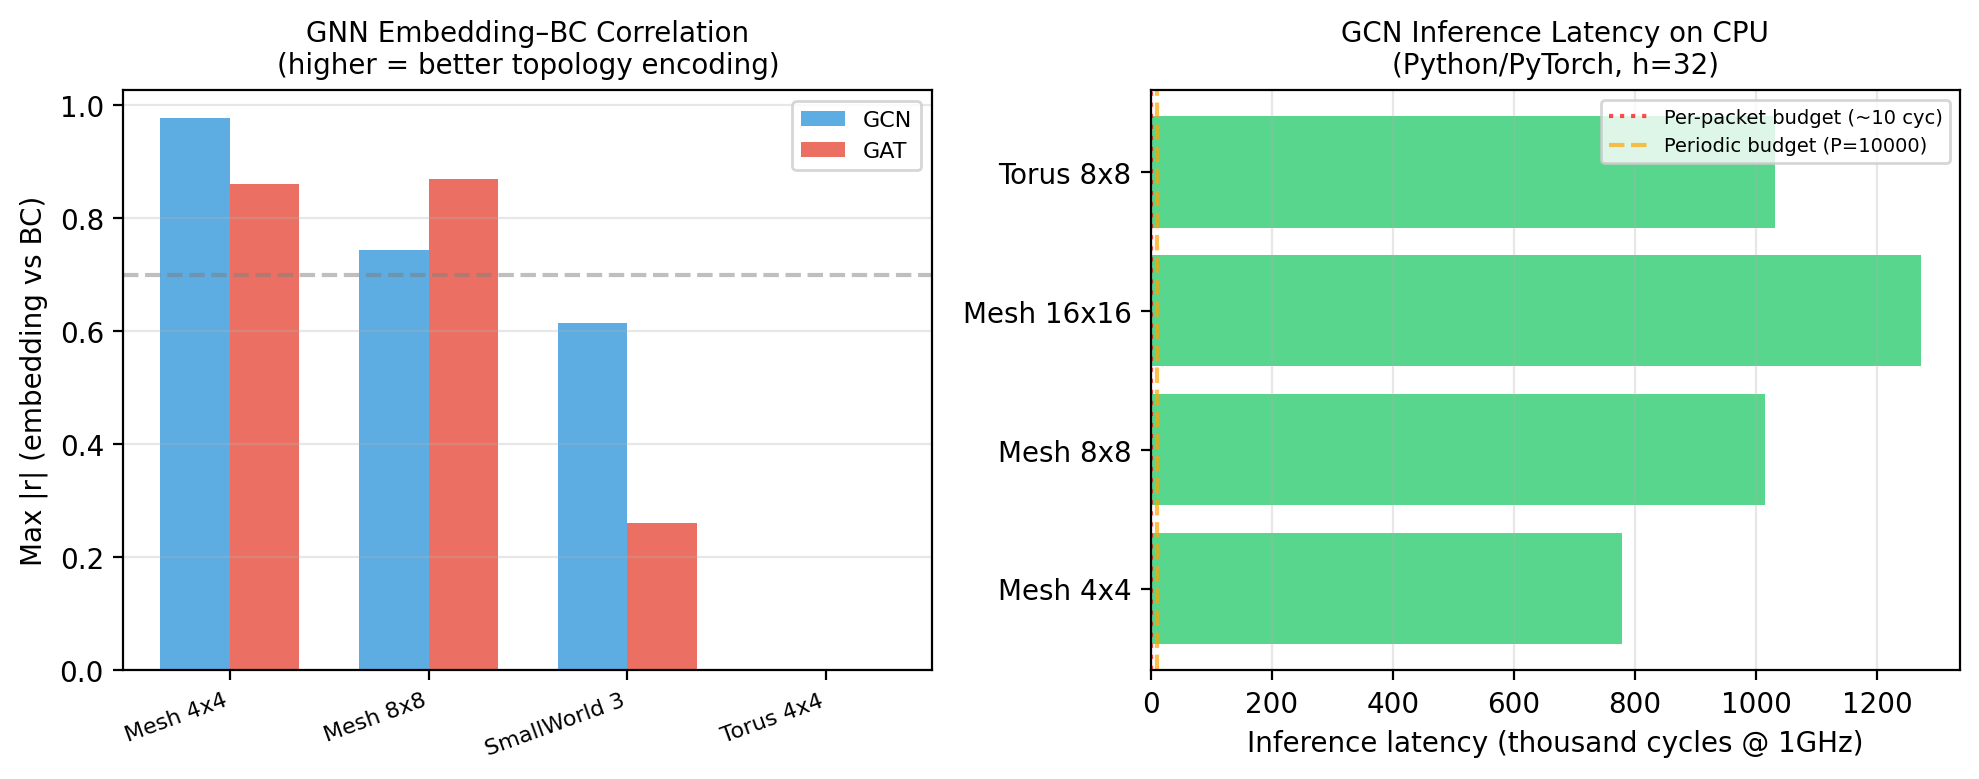
\includegraphics[width=0.85\textwidth]{gnn-results-summary.png}
\caption{Trái: Tương quan GNN embedding--BC. Phải: Inference latency
đo được trên CPU (Python/PyTorch).}
\label{fig:gnn-summary}
\end{figure*}

\subsection{Tổng quát hóa giữa các Topology}

\textbf{Thiết lập:} GCN (hidden=32) và GAT (hidden=16, heads=4) được
huấn luyện 500 epochs trên Mesh $4\times4$, đánh giá trên Mesh $8\times8$.

\begin{table}[h]
\centering
\caption{Dự đoán BC qua các topology (huấn luyện trên Mesh $4\times4$)}
\label{tab:generalization}
\resizebox{\columnwidth}{!}{%
\begin{tabular}{lcccr}
\toprule
\textbf{Test Topology} & \textbf{Model} & \textbf{MSE} & \textbf{R$^2$} & \textbf{Pearson $r$} \\
\midrule
Mesh $8\times8$ & GCN & 0.038 & $-16.83$ & \textbf{0.958} \\
Mesh $8\times8$ & GAT & 0.072 & $-33.00$ & \textbf{0.972} \\
Small-World & GCN & 0.004 & $-1.02$ & 0.385 \\
\bottomrule
\end{tabular}%
}
\end{table}

Trên Mesh $8\times8$, R$^2$ âm kết hợp với Pearson $r \approx 0.96$
cho thấy: model học được \emph{thứ tự tương đối} của các node (node nào
quan trọng hơn) nhưng không dự đoán được \emph{giá trị BC tuyệt đối}.

\textbf{Nhận xét:} Tương quan thứ tự cao ($r\approx0.96$) gợi ý rằng
GNN representations có thể chuyển giao pattern cấu trúc giữa các topology.
R$^2$ âm chỉ ra scaling tuyệt đối phụ thuộc topology---cần normalization
hoặc fine-tuning.

\subsection{Phân tích Inference Latency}

Chúng tôi đo inference latency của GNN trên CPU để đánh giá khả thi
dưới ràng buộc thời gian của NoC (mỗi quyết định cần $<$10 cycles).

\begin{table}[h]
\centering
\caption{Inference latency GNN trên CPU (Python/PyTorch)}
\label{tab:latency}
\resizebox{\columnwidth}{!}{%
\begin{tabular}{lccr}
\toprule
\textbf{Topology} & \textbf{Model} & \textbf{Latency ($\mu$s)} & \textbf{Cycles @ 1 GHz} \\
\midrule
Mesh $4\times4$ & GCN h=32 & 778 & 778,000 \\
Mesh $8\times8$ & GCN h=32 & 1,015 & 1,015,000 \\
Mesh $8\times8$ & GAT h=32 & 1,491 & 1,491,000 \\
Mesh $16\times16$ & GCN h=32 & 1,273 & 1,273,000 \\
\bottomrule
\end{tabular}%
}
\end{table}

Latency từ 778 $\mu$s đến 1,491 $\mu$s ($0.8$--$1.5$ triệu cycles ở 1 GHz).
Phiên bản C++ optimized ước tính giảm 1--2 orders of magnitude.

\textbf{Nhận xét:} Per-packet GNN inference là bất khả thi. Kết quả này
trực tiếp thúc đẩy giải pháp tối ưu định kỳ: với $P=10^5$ cycles và
inference optimized ($10^4$--$5\times10^4$ cycles), overhead là 10--50\%.

\subsection{Phân tích Scalability}

Đo inference time GCN từ $4\times4$ (16 nodes) đến $16\times16$ (256 nodes).

\begin{figure}[h]
\centering
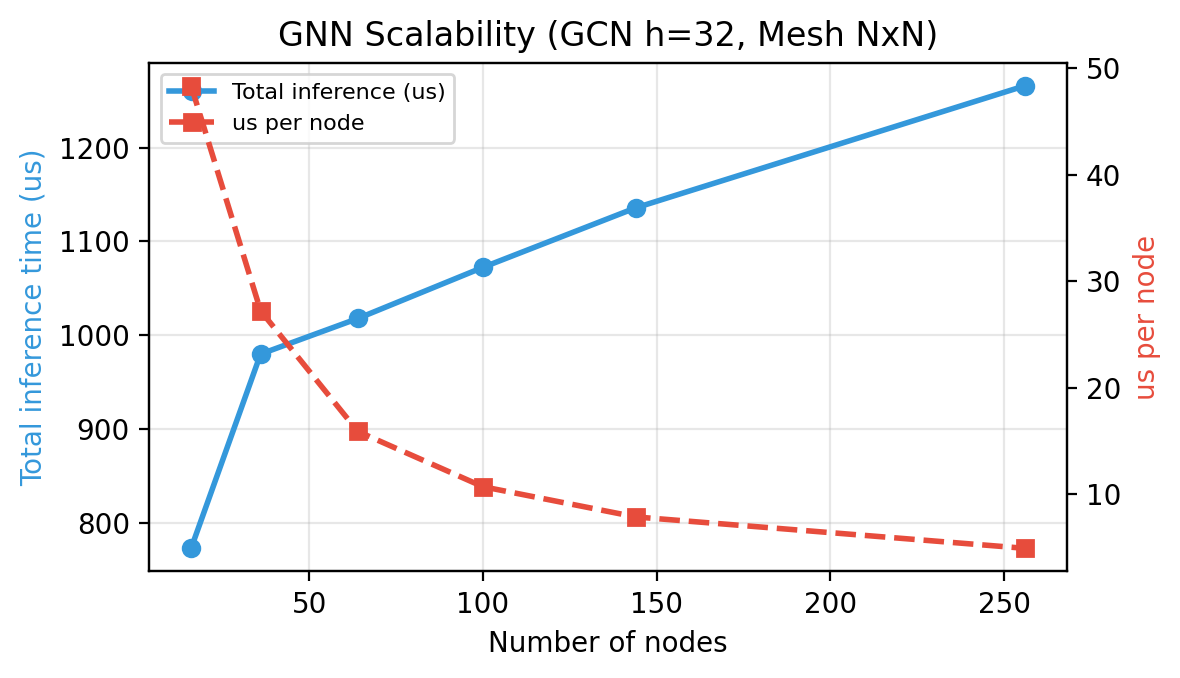
\includegraphics[width=0.85\columnwidth]{gnn-scalability.png}
\caption{GCN inference time scale O(N) với số nodes.}
\label{fig:scalability}
\end{figure}

Inference time tăng từ 773 $\mu$s (16 nodes) lên 1,266 $\mu$s (256 nodes).
Chi phí per-node giảm từ 48.3 xuống 4.9 $\mu$s/node.

\textbf{Nhận xét:} O(N) scaling dự đoán được, không bùng nổ.

% ══════════════════════════════════════════════════════════════
\section{Thảo luận}
\label{sec:discussion}
% ══════════════════════════════════════════════════════════════

\subsection{Hàm ý cho tối ưu định kỳ}

Inference latency ($10^5$--$10^6$ cycles) khẳng định per-packet GNN là
bất khả thi. Tuy nhiên, tương quan GNN-BC cao ($|r|=0.978$) cho thấy
GNN representations mang thông tin topology hữu ích. Với periodic update
$P=10^5$ cycles và optimized inference ($10^4$--$5\times10^4$ cycles),
overhead là 10--50\%.

\subsection{Thách thức tổng quát hóa}

GNN representations tổng quát hóa một phần (Pearson $r$ cao) nhưng
scale tuyệt đối phụ thuộc topology. Hai hướng: (1) topology-aware
normalization, (2) fine-tuning strategies.

\subsection{Hạn chế}

\begin{enumerate}
    \item \textbf{Static graph analysis:} Chưa có dynamic NoC state.
    \item \textbf{Chưa tích hợp routing simulation:} Cần cycle-accurate
    simulator để đánh giá end-to-end.
    \item \textbf{CPU-only measurements:} Trên server ARM, không phải
    embedded processor.
    \item \textbf{Chưa có RTL validation.}
    \item \textbf{Topology scope:} Chỉ 2D regular topologies.
\end{enumerate}

\subsection{Nguy cơ về tính giá trị}

\begin{itemize}
    \item Tương quan không đồng nghĩa với quan hệ nhân quả.
    \item Python overhead làm tăng latency đo được.
    \item Synthetic features còn đơn giản, thiếu tính thực tế.
\end{itemize}

% ══════════════════════════════════════════════════════════════
\section{Kết luận}
\label{sec:conclusion}
% ══════════════════════════════════════════════════════════════

Bài báo trình bày nghiên cứu khả thi về tối ưu định tuyến định kỳ
cho NoC sử dụng Graph Neural Networks. Ba kết quả thực nghiệm sơ bộ:

\begin{enumerate}
    \item GNN embeddings tương quan mạnh với BC ($|r|$ lên đến 0.978).
    \item Tổng quát hóa giữa các topology thành công một phần
    (Pearson $r \approx 0.96$).
    \item Inference latency ($\approx 10^6$ cycles) khẳng định
    periodic optimization là cần thiết.
\end{enumerate}

\textbf{Hướng phát triển:} (1) tích hợp GNN routing vào cycle-accurate
simulator; (2) phát triển topology-aware normalization; (3) đánh giá
quantized models trên embedded processors; (4) mở rộng sang irregular
topologies.

% ══════════════════════════════════════════════════════════════
% REFERENCES
% ══════════════════════════════════════════════════════════════

\begin{thebibliography}{99}

\bibitem{dyad2004} J. Hu and R. Marculescu, ``DyAD -- smart routing for networks-on-chip,'' \textit{Proc. DAC}, 2004.

\bibitem{wang2022maar} Y. Wang et al., ``MAAR: Multi-agent adaptive routing for network-on-chip,'' \textit{IEEE Trans. Computers}, vol. 71, no. 8, pp. 1878--1891, 2022.

\bibitem{deepnr2022} R. R. RS et al., ``DeepNR: An adaptive deep reinforcement learning based NoC routing algorithm,'' \textit{Microprocessors and Microsystems}, vol. 92, 104499, 2022.

\bibitem{g-routing2023} H. Wei, Y. Zhao, and K. Xu, ``G-Routing: Graph neural networks-based flexible online routing,'' \textit{IEEE Network}, 2023.

\bibitem{drl-gnn2019} P. Almasan et al., ``Deep reinforcement learning meets graph neural networks: Exploring a routing optimization use case,'' \textit{arXiv:1910.07421}, 2019.

\bibitem{graphnoc2024} G. S. Malik and N. Kapre, ``GraphNoC: Graph neural networks for application-specific FPGA NoC performance prediction,'' \textit{Proc. FPT}, IEEE, 2024.

\bibitem{noctopus2026} V. Iyengar, V. H. Bui, and S. Das, ``NOCTOPUS: Network-on-Chip topology optimization and prediction using simulation-data,'' \textit{Neural Computing and Applications}, Springer, 2026.

\bibitem{mirhoseini2021} A. Mirhoseini et al., ``A graph placement methodology for fast chip design,'' \textit{Nature}, vol. 594, pp. 207--212, 2021.

\bibitem{ebrahimi2019} M. Ebrahimi, M. Daneshtalab, and J. Plosila, ``Regional-based routing for network-on-chip,'' \textit{IEEE TCAD}, 2019.

\bibitem{garnn2023} H. Zhang et al., ``GARNN: Graph attention routing for network-on-chip,'' \textit{Proc. DATE}, 2023.

\bibitem{slimnoc2018} M. Besta et al., ``Slim NoC: A low-diameter on-chip network topology for high energy efficiency and scalability,'' \textit{Proc. ASPLOS}, ACM, 2018.

\bibitem{sparsehamming2023} P. Iff et al., ``Sparse Hamming Graph: A customizable network-on-chip topology,'' \textit{Proc. DAC}, 2023.

\bibitem{gatv2} S. Brody, U. Alon, and E. Yahav, ``How attentive are graph attention networks?'' \textit{Proc. ICLR}, 2022.

\bibitem{ppo2017} J. Schulman et al., ``Proximal policy optimization algorithms,'' \textit{arXiv:1707.06347}, 2017.

\bibitem{duato1996} J. Duato, ``A necessary and sufficient condition for deadlock-free routing in cut-through and store-and-forward networks,'' \textit{IEEE Trans. Parallel and Distributed Systems}, vol. 7, no. 8, pp. 840--854, 1996.

\bibitem{pyg2019} M. Fey and J. E. Lenssen, ``Fast graph representation learning with PyTorch Geometric,'' \textit{ICLR Workshop}, 2019.

\bibitem{networkx2008} A. Hagberg, P. Swart, and D. S. Chult, ``Exploring network structure, dynamics, and function using NetworkX,'' \textit{Proc. SciPy}, 2008.

\end{thebibliography}

\end{document}
